\chapter{Vyhodnotenie výsledkov}\label{chap:results}

Vyhodnotenie získaných výsledkov sme rozdelili na štyri časti. V prvej časti sme sa zamerali na detekciu, v druhej na sledovanie a v tretej na určenie významnosti. Posledná časť je venovaná výsledkom z klasifikácie.

\section{Detekcia reklám}

Nazačiatku sme natrénovali tri modely, ktoré mali pri tréningu rovnako nastavené parametre a líšili sa jedine verziou dát. Počet epoch bol nastavený na 128, veľkosť dávky na 16 a ostatné parametre boli ponechané s prednastavenými hodnotami. Najlepšie počiatočné váhy, s ktorými dokázal server spracovať mali označenie YOLOv8large. Váhy s väčším počtom parametrov zlyhali pri výpočtoch kvôli nedostatku pamäte na grafickej karte. Dĺžka trénovanie jednej epochy bola približne 20 minút pre pôvodnú verziu dát a 10 minúť pre obe odfiltrované verzie.

Na vyhodnotenie modelu sa počíta pomer medzi prienikom a zjednotením detekovanej plochy so skutočnou plochou objektu. Táto hodnota sa označuje skratkou IoU (Intersection over Union). Nastavením požadovanej hodnoty pre IoU sa určujú tri základné stavy detekcie:

\begin{itemize}
  \item skutočne pozitívna detekcia (true positive, TP)
  \item falošne pozitívna detekcia (false positive, FP)
  \item falošne negativna detakcia (false negative, FN)
\end{itemize}

Na obrázku \ref{img:ious} sú znázornené všetky tri situácie s prahovou hodnotou 0.5. Pokiaľ by sme zmenili hodnotu prahu na 0.9, tak aj v prvom prípade by bola detekcia vyhodnotená ako FP.

\begin{figure}[ht]
    \centering
    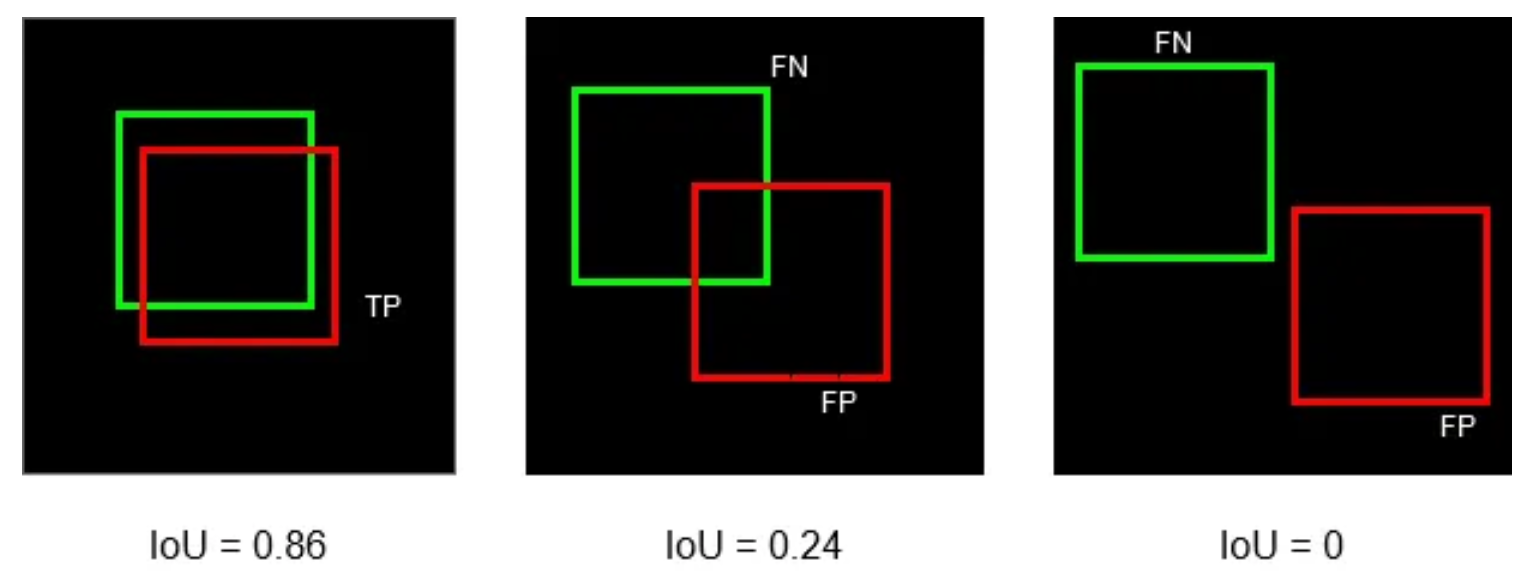
\includegraphics[width=1\textwidth]{images/05/ious.png}
    \caption{Vyhodnotenie detekcie podľa prahovej hodnoty IoU.}
    \label{img:ious}
\end{figure}

Na základe takýchto elementárnych vyhodnotení sa počíta viacero metrík. Metrika precision určuje koľko detekcií bolo skutočne pozitívnych a metrika recall určuje koľko skutočne pravdivých označení bolo odhalených skutočne pozitívnou detekciou.

%\begingroup
%\begin{equation}
%Precision = \frac{|TP|}{|TP| + |FP|}
%\label{e:DetPr}
%\end{equation}
%
%\begin{equation}
%Recall = \frac{|TP|}{|TP| + |FN|}
%\label{e:DetRe}
%\end{equation}
%
%\begin{equation}
%DetA = \frac{|TP|}{|TP| + |FN| + |FP|}
%\label{e:DetA}
%\end{equation}
%\endgroup

Presnosť a citlivosť je okrem prahovej hodnoty IoU ovplyvnená ešte prahovou hodnotou istoty (confidence), ktorá je vypočítaná pre každú detekciu. Confidence hodnota určuje istotu modelu, že je daná detekcia správna. Model zaznačí len také detekcie, ktoré majú istotu vyššiu ako je nastavená prahová hodnota.

Závislosť medzi presnosťou a citlivosťou sa znázorňuje pomocou grafu. Obsah plochy pod krivkou je označovaný ako mAP (mean Average Precision). Výsledná hodnota mAP50 je priemer presnosti pre hodnotu prahu IoU = 0.5. V prípade metriky mAP50-95 je priemer počítaný pre prah IoU od 0.5 do 0.95.

V tabuľke \ref{table:test1} je každý model otestovaný na testovacej sade príslušnej verzie. Tým, že má každá verzia inú testovaciu sadu, nemôžme povedať, ktorý model je najlepší. Pre lepšie otestovanie modelov sme mali pripravenú testovaciu vzorku obrázkov, tvorenú zo snímok z experimentálneho merania. Vyhodnotenie modelov na testovacej vzorke v tabuľke \ref{table:test2} ukazuje, že model M3 dosahuje najlepšie výsledky. Model M1, ktorý na testovacej sade dosiahol výrazne horšie výsledky, bol napokon porovnateľný s ostatnými modelmi pri vyhodnotení na spoločnej testovacej vzorke. Metriky boli počítané pre prahovú hodnotu IoU = 0.5 s istotou väčšou ako 0.3.

\newpage

\begin{table}[ht]
\centering
\begin{tabular}{ |c c c c c| }
\hline
model & presnosť & citlivosť & mAP50 & mAP50-95 \\
\hline
M1  & 0.473 & 0.352	& 0.327	& 0.195 \\
M2  & 0.554	& 0.505	& 0.492	& 0.311 \\
M3  & 0.577	& 0.504	& 0.503	& 0.324 \\
\hline
\end{tabular}
\caption{Výsledky z trénovania. Modely sú označené číslom podľa verzie dát.}
\label{table:test1}
\end{table}

\begin{table}[ht]
\centering
\begin{tabular}{ |c c c c c|  }
\hline
model & presnosť & citlivosť & mAP50 & mAP50-95 \\
\hline
M1  & 0.692	& 0.522	& 0.615	& 0.446 \\
M2  & 0.659 & 0.565 & 0.653 & 0.467 \\
M3  & 0.715 & 0.541 & 0.656 & 0.480 \\
\hline
\end{tabular}
\caption{Výsledky tých istých modelov na spoločnej testovacej vzorke obrázkov.}
\label{table:test2}
\end{table}

Na obrázku \ref{img:dt7} je vizualizácia detekcií z vybranej snímky. Označenie detekcie má číselnú hodnotu, ktorá určuje istotu detekcie. V tomto prípade vidíme detekciu vo väčšej vzdialenosti a aj detekciu reklamy s výrazným prekrytím.

\begin{figure}[ht]
    \centering
    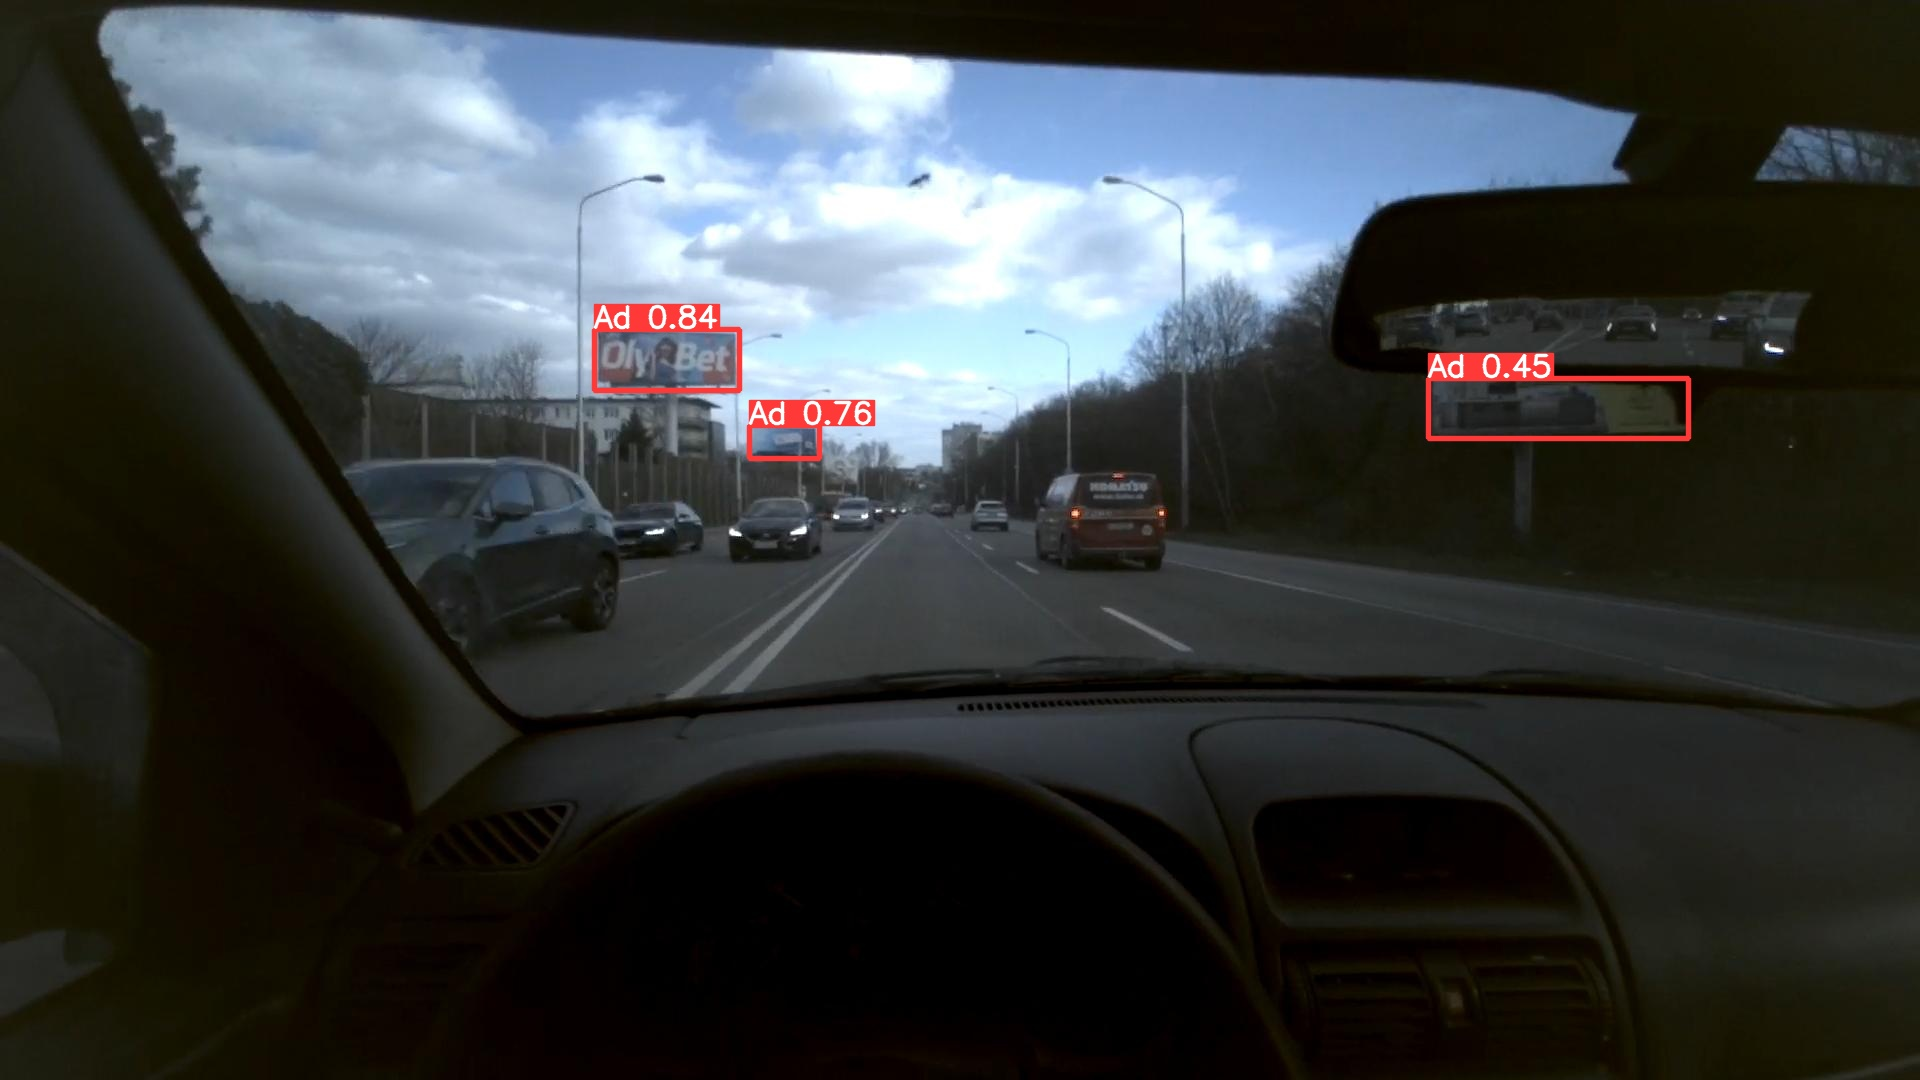
\includegraphics[width=1\textwidth]{images/05/120.jpg}
    \caption{Ukážka detekcií zo snímky s väčším počtom reklám.}
    \label{img:dt7}
\end{figure}

\section{Sledovanie reklám}

Na vyhodnotenie sledovania objektov, existuje viacero zaužívaných metrík. Rozhodli sme sa použiť metriku so skratkou HOTA (Higher Order Tracking Accuracy) \cite{hota}, ktorá sa kladá z menších častí, podľa ktorých sa dajú vyhodnotiť tri aspekty sledovania:

\begin{itemize}
    \item lokalizácia
    \item detekcia
    \item asociácia
\end{itemize}

Lokalizácia a detekcia sa meria rovnako ako pri testovaní detektorov. Asociácia meria ako dobre sa podarilo spojiť detekciu s referenciou. Podobne ako pri detekcii môžu nastať tri stavy, ktoré určujú správnosť asociácie:

\begin{itemize}
  \item skutočne pozitívna asociácia (true positive association, TP)
  \item falošne pozitívna asociácia (false positive association, FP)
  \item falošne negativna asociácia (false negative association, FN)
\end{itemize}

% https://jonathonluiten.medium.com/how-to-evaluate-tracking-with-the-hota-metrics-754036d183e1
% https://arxiv.org/pdf/2009.07736.pdf

Obrázok \ref{cite:usecase} vysvetľuje koncepty TPA, FPA a FNA na objekte, ktorý je označený v červenom štvorci. Zelená farba označuje stav TPA, v ktorom je predikovaná referencia rovnaká so skutočnou referenciou objektu. Žltá farba označuje FPA, ktorá je v prvom prípade zapríčinená FP detekciou a v druhom prípade tým, že asociácia vstupuje to trajektórie iného objektu. Hnedá farba označuje FNA v prípade, kde sa nepodarilo zachytiť skutočnú časť trajektórie.

\begin{figure}[ht]
    \centering
    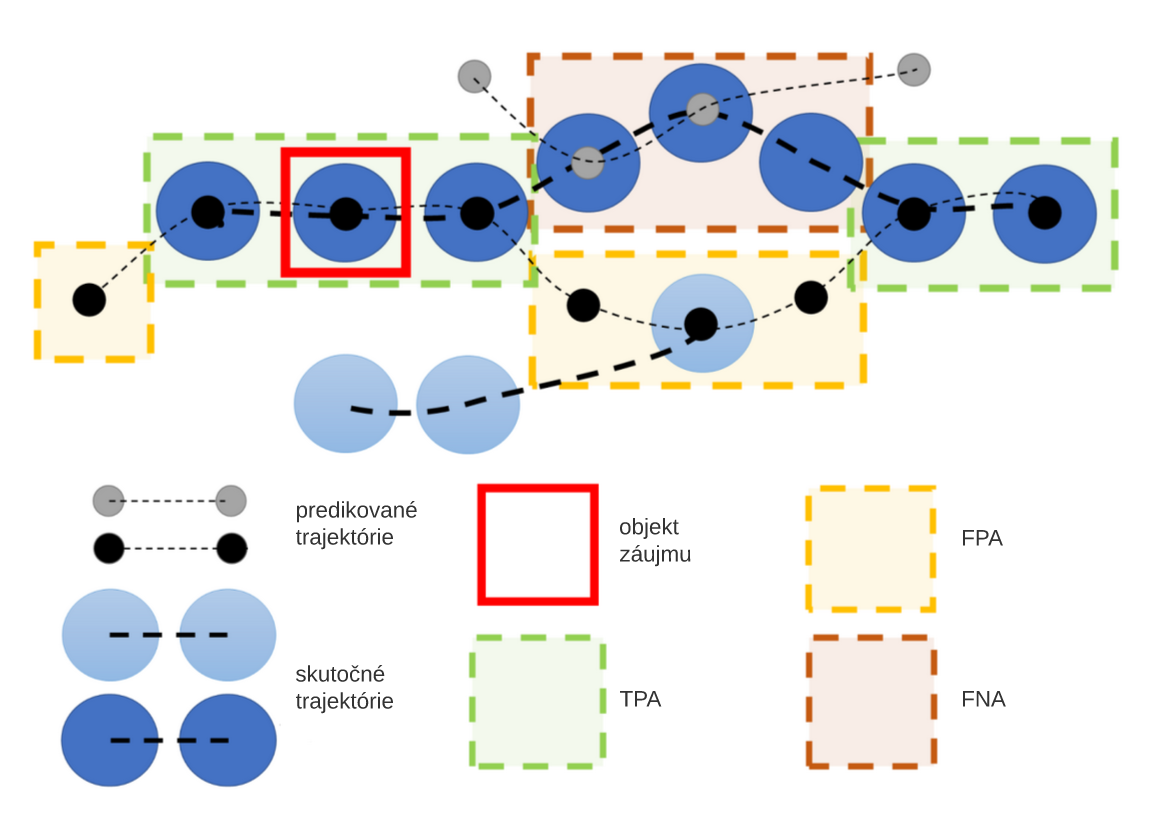
\includegraphics[width=0.7\textwidth]{images/05/usecase.png}
    \caption{Vizualizácia všetkých možností, ktoré môžu vzniknúť pri sledovaní \cite{hota}.}
    \label{img:usecase}
\end{figure}

Geometrickým priemerom detekcie a asociácie je vypočítaná hodnota HOTA. Táto formulácia zabezpečuje, že detekcia aj asociácia sú na rozdiel od mnohých iných metrík sledovania rovnomerne vyvážené a že konečné skóre je niekde medzi nimi.

Každá sledovacia metóda bola spustená viackrát s rôznou konfiguráciou. Najlepšie výsledky pre každú metódu sú zapísané v tabuľke \ref{table:hota1}.
\\
\begin{table}[ht]
\centering
\begin{tabular}{|l l l l l l l l l|}
 \hline
metóda & HOTA & DetPr & DetRe & DetA & AssPr & AssRe & AssA & LocA \\ [0.5ex]
 \hline
OC-SORT & 37.936 & 58.479 & 54.554 & 40.455 & 74.731 & 42.579 & 35.638 & 88.581 \\ [0.1ex]
DeepOC-SORT & 39.152 & 63.357 & 54.578 & 42.673 & 70.841 & 42.888 & 35.937 & 88.932 \\ [0.1ex]
StrongSORT & 39.152 & 63.357 & 54.578 & 42.673 & 70.841 & 42.888 & 35.937 & 88.932 \\ [0.1ex]
BotSORT & 27.141 & 40.139 & 38.162 & 24.812 & 40.389 & 56.746 & 29.729 & 87.301 \\ [0.1ex]
ByteTrack & 27.760 & 37.434 & 34.147 & 22.085 & 57.887 & 47.258 & 34.957 & 88.027 \\ [0.1ex]
 \hline
\end{tabular}
\caption{TODO, výsledky 4.}
\label{table:hota1}
\end{table}
\\
TODO We can see how well methods perform in each of the dimensions of detection (x-axis) and association (y-axis) separately, with the curves in the background showing how the overall HOTA score increases as both detection and association scores increase. We can go further than just comparing detection and association. Because they are both naturally decomposable into one component.
\begin{figure}[ht]
    \centering
    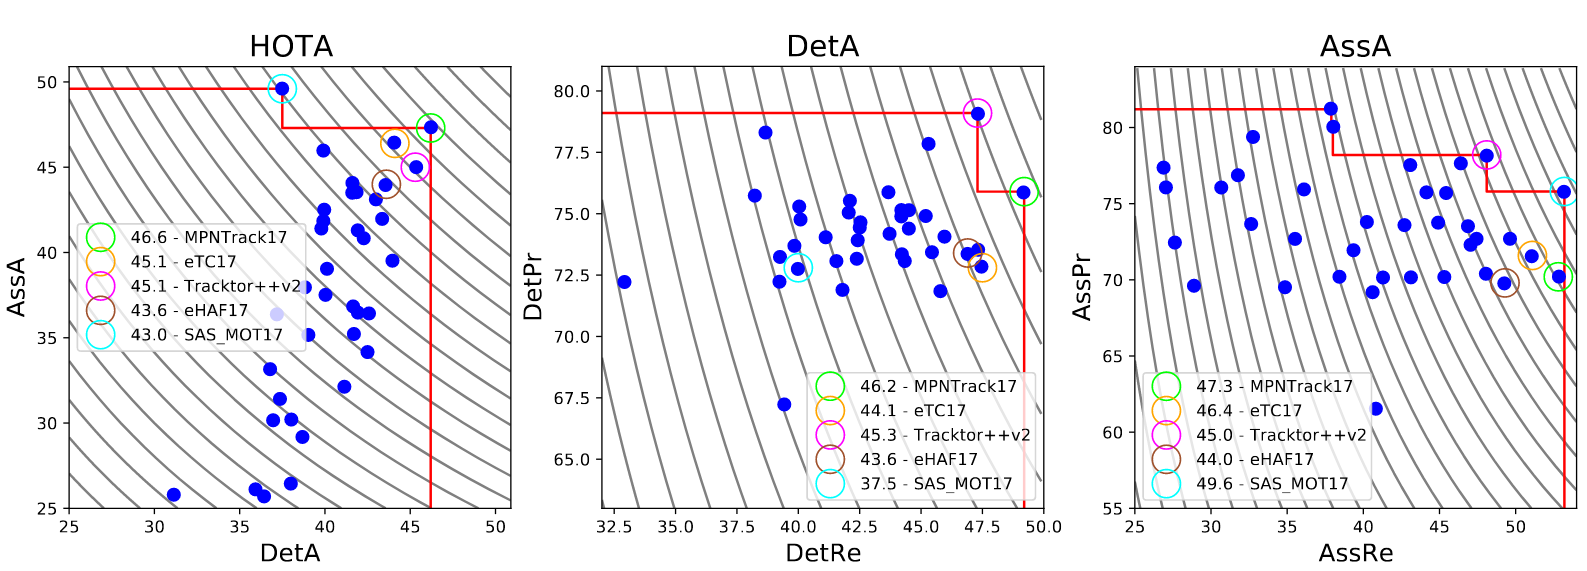
\includegraphics[width=1\textwidth]{images/05/compare.png}
    \caption{.}
    \label{img:road}
\end{figure}

TODO Tu je vizualizácia sledovania reklám z videa. Na pravej strane obrázka je metóda X a na ľavej Y. Snímky sú v tomto prípade zachytené každých 10 snímok a vidíme, že metóda Y nepriradila referenciu po oklúzii správne.
\begin{figure}[ht]
    \centering
    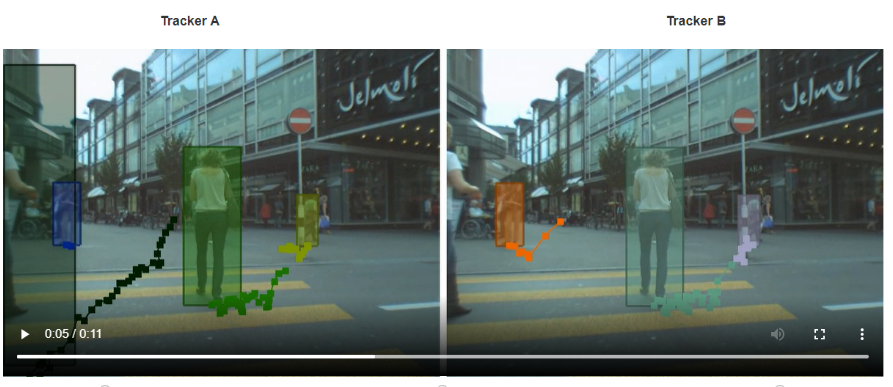
\includegraphics[width=1\textwidth]{images/05/vs.png}
    \caption{.}
    \label{img:road}
\end{figure}

\section{Významnosť reklám}

Dokopy bolo na zvolenej trase nájdených 145 reklám, ktoré sa podľa počtu prienikov rozdelili do štyroch kategórií. V tabuľke \ref{table:cat} je pre každú kategóriu zapísané časové rozmedzie korešpondujúce počtu snímok s prienikom, počet reklám vyhodnotených do príslušnej kategórie a priemerný počet účastníkov, ktorý sa na reklamu danej kategórie pozreli.
% todo pridať obrázok, kde je fixácia
\\
\begin{table}[ht]
\centering
\begin{tabular}{|c c c c|}
 \hline
 kategória &	rozmedzie &	počet reklám &	počet účastníkov \\ [0.5ex]
 \hline
slabá &	0 ms &	27 &	- \\ [0.1ex]
nízka &	1-249 ms &	66 &	2.95 \\ [0.1ex]
stredná &	250-499 ms &	18 &	5.11 \\ [0.1ex]
vysoká &	500+ ms &	3 &	2 \\ [0.1ex]
 \hline
\end{tabular}
\caption{TODO, výsledky 5.}
\label{table:cat}
\end{table}



\section{Klasifikácia reklám}

Jedna.

\newpage

Dva.

\newpage

Tri.

%If your use-case contains many occlussions and the motion trajectiories are not too complex, you will most certainly benefit from updating the Kalman Filter by its own predicted state. Select the number of predictions that suits your needs here: https://github.com/mikel-brostrom/Yolov5_StrongSORT_OSNet/blob/b1da64717ef50e1f60df2f1d51e1ff91d3b31ed4/trackers/strong_sort/configs/strong_sort.yaml#L7
